% Activate the following line by filling in the right side. If for example the name of the root file is Main.tex, write
% "...root = Main.tex" if the chapter file is in the same directory, and "...root = ../Main.tex" if the chapter is in a subdirectory.
 
%!TEX root =  TNTinderSee.tex

Um den sprengstofftypischen Verbindung auf die Spur zu kommen, war es unabdinglich, an verschiedenen Orten Wasserproben zu nehmen. Die Probe muss dabei nicht etwa in unmittelbarer Nähe von Minen, Bomben o.ä. genommen werden, da sprengstofftypische Verbindungen typischerweise auch noch an weiter entfernten Positionen nachzuweisen sind. Wir entschieden uns für Probenaufnahmen in der Nähe des ehemaligen Ankerplatzes und des Unglücksortes der 1945 gesunkenen Schute.

\subsubsection{Technische Beschreibung und Durchführung an Board}
Die Wasserbeprobung ist relativ simpel. Wir hatten dafür ein Plastikrohr mit Deckeln, welche mithilfe von zwei Gummis offen gehalten wurden. Das Rohr wurde ins Wasser gelassen, jeweils abgestimmt auf die Wassertiefe Tiefe abzüglich eines Meters, so dass aufgewirbelter Dreck oder Algen nicht im Weg waren. Sobald sich das Plastikrohr an der richtigen Stelle befand, wurde ein kleines metallenes \emph{Engelchen} dem Seil entlang, an welchem das Rohr befestigt war, in die Tiefe geschickt. Das Engelchen war aufgrund von seinem Material relativ schwer, wodurch sich die Gummis an dem Rohr lösten und die Deckel zu gingen. Danach musste die Probe nur noch hoch gezogen werden.

Sobald sich die Probe wieder auf dem Boot befand, konnten wir weiter zum nächsten Standpunkt fahren. Auf dem Boot ging dann allerdings erst die richtige Arbeit los, nämlich aus der rohen Wasserprobe eine zu machen, aus welcher man auch Informationen ziehen konnte. An dem Rohr befand sich ein kleines Ventil, wodurch wir das Wasser langsam und kontrolliert in einen Messbecher laufen lassen konnten. Mit viel Feingefühl versuchten wir genau 1000ml zu bekommen. Es würde keinen großen Unterschied machen, wenn es mehr oder weniger wäre, allerdings hat uns das Abmessen einiges an Rechnen erspart. 

Das abgemessene Wasser wurde anschliessend durch einen selbst gebauten Trichter in ein \emph{Blood Bag} gefüllt, solche wie man auch bspsw. bei Operationen im Krankenhaus findet, um Blut zu lagern. In unserem Fall war dies allerdings nur ein Zwischenschritt. 
An dem Blood Bag befestigten wir einen kleinen Schlauch mit einem Filter, durch dass das Wasser gelassen wurde. Im Anschluss an den Filter, welcher lediglich Schmutzpartikel aus dem Wasser filterte, befand sich ein kleines Teströhrchen mit einer Art Granulat. Dieses war nach unten hin offen, da das fertig durchgelaufene Wasser unbrauchbar für uns war, weshalb wir es einfach langsam abtropfen lassen konnten.

Die eigentliche Magie war nun das Geschehen in dem Granulat. Dieses dient dazu, schadstoffähnliche Verbindungen aus dem Wasser zu filtern und zu speichern. 

\subsubsection{Probenpräparation am GEOMAR}
Die Teströhrchen haben wir anschließend mit ins Geomar nach Kiel genommen. Dort haben wir die Proben für den Ionenchromatographen präpariert, indem wir eine definierte Menge von destilliertem Wasser über das Granulat haben laufen lassen. Anschließend wurden die Proben mit einem Verdünnungsmittel auf 2ml aufgefüllt. Diese nun fertige Probe wurde dann auf Rückstände sprengstofftypischer Verbindungen analysiert.
\begin{figure}[]
    \centering
    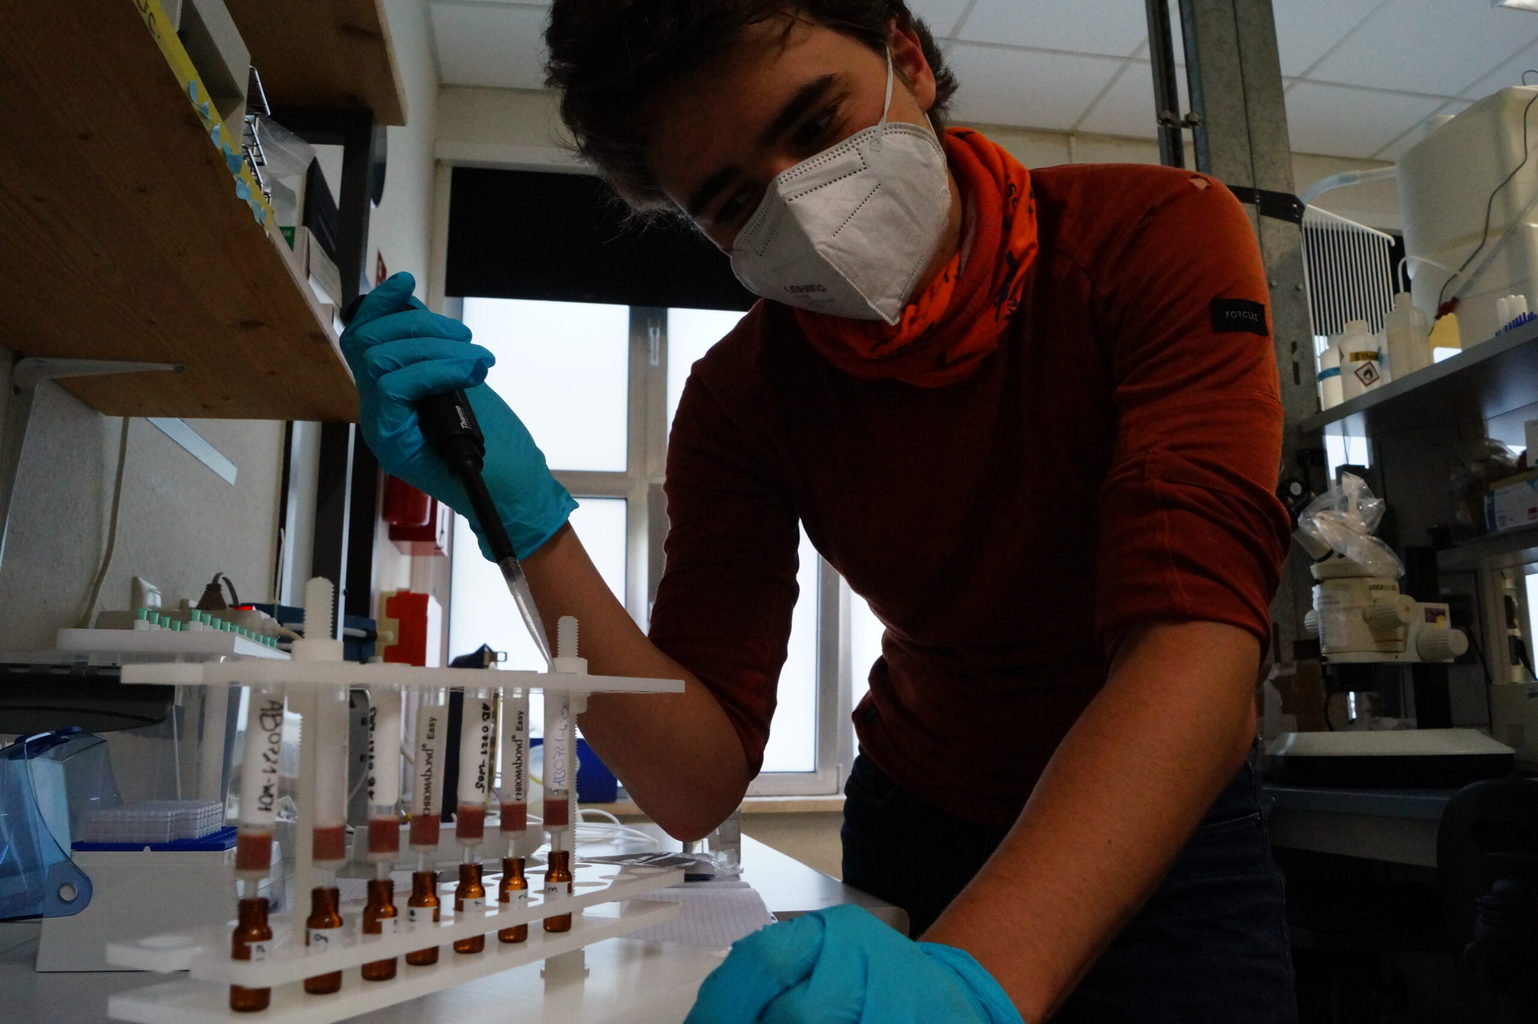
\includegraphics[width=0.8\linewidth]{Bilder/DSC05766-scaled.jpg}
    \caption{Vorbereitung der Wasserproben für den Ionenaustauschchromatographen}
    \label{fig:praep}
\end{figure}